\section{Results on the Benchmark}
\label{sec:results}
% SWEVO extension: the coefficient sweep (Fig. fig:S-csweep, Table tab:S-csweep), the PSO-dynamics diagnostic
% (Fig. fig:D-psodyn), the average ranks (Fig. fig:ranks), the wake loss versus N (Fig. fig:wakeloss), the equivalence
% curve (Fig. fig:equiv-curve) and the equivalence and heterogeneity tables (tab:X-equiv-levels, tab:X-heterogeneity)
% were moved here from the supplementary material (log: optA/sw/moved.md).
\makeatletter
% Capture the generated floats of the diagnostics and of the inference robustness checks; figures are stored like the
% tables (by their first \label) and placed with \swResFigure. The capture is global and typesets nothing.
\begingroup
\RenewEnviron{figure}[1][]{\supp@store}\RenewEnviron{figure*}[1][]{\supp@store}%
\CaptureSuppTables{analysis/mpce_supp_diag.tex}%
\CaptureSuppTables{analysis/mpce_supp_inference.tex}%
\endgroup
\newcommand{\swResFigure}[1]{\@ifundefined{supp@body@#1}{\par\noindent\TBD{generated figure \detokenize{#1} not found}\par}{%
  \@ifundefined{supp@used@#1}{\global\@namedef{supp@used@#1}{}%
    \begin{figure*}[!t]\@nameuse{supp@body@#1}\end{figure*}}{}}}
% Reference to a label that is either in the main text or (prefix S-) in the supplementary material: the generated
% captions use the supplement's label names; a label placed in the main text resolves there, any other one in the
% supplement (\swResRefs makes \ref behave like this inside a group). Aliases: supplement names of main-text labels.
\@namedef{swres@alias@prop:S-pso-stability}{prop:pso-stability}
\protected\def\swResRef#1{\@ifundefined{swres@alias@#1}%
  {\@ifundefined{r@#1}{\swres@origref{S-#1}}{\swres@origref{#1}}}%
  {\swres@origref{\@nameuse{swres@alias@#1}}}}
\let\swres@origref\ref
\newcommand{\swResRefs}{\let\ref\swResRef}
% notes of tab:X-heterogeneity: long \multicolumn{8}{l} rows, set as wrapped paragraphs (as in the supplement)
\newcommand{\swResWrapNotes}{\let\swres@mc\multicolumn
  \def\multicolumn##1##2##3{\swres@mc{##1}{p{0.9\textwidth}}{##3}}}
\makeatother
This section reports the 68 benchmark cases (\NRunsBenchmark{} runs of 6,030 evaluations, random starts, 15$^\circ$ rose; per case: Tables~\ref{S-tab:res-1-500}--\ref{S-tab:res-2-1000}). It first shows how strongly the configuration of the PSO baseline changes the comparison and why (Section~\ref{sec:psosetting}), then compares the eight methods over all cases (Section~\ref{sec:overall}), and finally examines the one comparison that the average does not settle, PSO-VNS against the well-configured PSO from which it starts (Section~\ref{sec:psovns-pso}).

\subsection{Effect of the Baseline Setting}
\label{sec:psosetting}
\label{sec:baseline}
\IfFileExists{analysis/mpce_tab_baseline.tex}{%% generated by mpce_results.py -- do not edit by hand
\begin{table}[!t]
\centering
\caption{Effect of the PSO Setting on the Comparison of the Previous Study's Methods (68 Cases, 6,030 Evaluations): Average Rank (1 = Best) with the Old ($w=0.7$, $c_1=c_2=2$) and the Constriction Setting, and Run-Level W/T/L of the Salp-Swarm Hybrids against PSO}
\label{tab:baseline}
\footnotesize\setlength{\tabcolsep}{4pt}
\begin{tabular}{lcc}
\toprule
& \multicolumn{2}{c}{PSO setting} \\
\cmidrule(lr){2-3}
Method & Old & Constriction \\
\midrule
LX-SSA-VNS & 2.65 & 3.41 \\
SSA-VNS & \textbf{1.99} & 2.77 \\
LX-SSA & 5.65 & 6.06 \\
SSA & 4.81 & 5.34 \\
PSO & 5.04 & \textbf{1.53} \\
DE & 6.99 & 7.03 \\
VNS & 3.59 & 4.15 \\
MS-SLSQP & 5.28 & 5.71 \\
\midrule
PSO position & 5 & 1 \\
LX-SSA-VNS vs.\ PSO (W/T/L) & 35/33/0 & 0/21/47 \\
SSA-VNS vs.\ PSO (W/T/L) & 41/27/0 & 0/22/46 \\
\bottomrule
\multicolumn{3}{p{0.95\columnwidth}}{Ranks: feasibility-aware rule (fewer than 15 of 30 feasible runs in a case = ranked last); bold: best average rank. W/T/L: cases in which the hybrid is significantly better / not different / worse than PSO (two-sided Wilcoxon signed-rank test, 30 seed-paired runs, Holm-adjusted over the seven comparisons of the hybrid in each case, $\alpha=0.05$).}
\end{tabular}
\end{table}
}{}
The old setting lies beyond the order-2 (variance) stability boundary~\eqref{eq:poli}. Run on the same cases, budget and seeds as the constriction setting~\eqref{eq:constriction}, it returns a feasible layout in only \NOldPSOFeas\% of the runs (fewer than 15 feasible runs in \NOldPSOBelowHalf{} cases), is significantly worse in \NOldPSOWorse{} of the 68 cases and never better, and has a mean wake loss \NOldPSODL{}~pp higher over the \NOldPSOCases{} cases in which both settings have at least 15 feasible runs. Both settings share the code, the population of 30, the zero initial velocities, the box repair (a clipped coordinate keeps its velocity; no velocity clamping) and, for every seed, the initial swarm; only the three coefficients differ, so every difference between the two columns of Table~\ref{tab:baseline} comes from the setting alone.
% CHECK-FINAL [C12]: pso_setting: constriction_vs_old L == 0, W >= 34 (editor cut C5 applied)

\begingroup\swResRefs\swResFigure{fig:D-psodyn}\endgroup
\emph{What goes wrong.} In instrumented reruns (clipping without velocity reset or clamping; Fig.~\ref{fig:D-psodyn} and Table~\ref{S-tab:D-psodyn}), its swarm contracts much less (final spread \NDSpreadRatio{} times, velocity \NDVelRatio{} times that of the constriction setting), \NDClipOld\% of the coordinates are clipped (constriction: \NDClipNew\%), and far fewer particle evaluations in the second half of a run are feasible (\NDFeasPartOld\% vs.\ \NDFeasPartNew\%). The reruns cover \NDDynCases{} cases $\times$ \NDDynSeeds{} seeds and reproduce the stored runs of the paper (Section~\ref{S-sec:S-diag}). The three panels of Fig.~\ref{fig:D-psodyn} show one chain of effects. With the constriction setting, the swarm spread around the global best $\mathbf G$ shrinks steadily, as expected for an order-2 stable setting whose limit variance in each coordinate is proportional to $(P^i_m-G_m)^2$ (Proposition~\ref{prop:pso-stability}): as the personal bests approach $\mathbf G$, the particles sample ever closer to it. With the old setting, the spread stays at a sizeable fraction of the farm radius for the whole run, and such steps keep carrying coordinates out of the square. Because a clipped coordinate keeps its velocity, it stays on the bound as long as its velocity points outward, and every evaluation with a coordinate at $\pm r$ violates the circular boundary unless the other coordinate is zero (Lemma~\ref{S-lem:S-clip}); consistent with this, the share of clipped coordinates stays high instead of decaying to almost zero. A swarm that samples this widely rarely hits the narrow feasible region of a dense layout: in the course of a run a growing share of the constriction swarm is feasible, whereas the old setting remains almost always infeasible, and most of its infeasible evaluations violate both constraints (a turbine outside the circle and a pair too close).
% CHECK-DIAG [D03] spread/|V| ratios ("contracts much less"); [D04] clipped share; [D05] feasible particle evaluations (iterations 101-200); [D07] most infeasible particle evaluations of the old setting violate both constraints; [D01] instrumented runs reproduce the stored runs

The final layouts tell a different story from the particle evaluations. Of the \NDStoredInfeasOld{} infeasible final layouts of the old setting (of \NDStoredRunsOld{} stored runs; $10^{-6}$~m rule of the paper), \NDStoredSpacingOnlyOld{} violate only the spacing constraint, \NDStoredBoundOnlyOld{} only the boundary and \NDStoredBothOld{} both; the constriction setting has none. This is a consequence of the penalty scaling in~\eqref{eq:penalty}: the boundary violation $g^{\rm b}_i=x_i^2+y_i^2-r^2$ is measured in m$^2$ and the spacing violation $g^{\rm s}_{ij}$ in m, so a turbine clearly outside the circle costs much more than two turbines slightly too close, and the best infeasible layout that $\mathbf G$ retains tends to lie inside the circle with a spacing violation. Most of the remaining boundary violations are a scaling effect as well: in \NDStoredTangentOld{} of the \NDStoredAnyBoundOld{} final layouts that violate the boundary, an outside turbine is pinned at the box near a point where the square touches the circle, where $g^{\rm b}_i$ is of second order in the other coordinate and hence cheap (Section~\ref{sec:constraints}). The infeasibility of the final layouts of the old setting is therefore mainly a spacing problem, not one of turbines left outside the farm; a penalty with normalized violations, e.g., $(\lVert\mathbf x_i\rVert-r)/r$ and $(\ell_{\min}-\ell_{ij})/\ell_{\min}$, would avoid both scaling effects.
% CHECK-DIAG [D06] infeasible finals of the old setting mostly spacing-only (224 of 286), boundary-only < spacing-only, constriction none; [D21] >= 90 % of boundary-violating finals pinned at the box (tangent point)

\begingroup\swResRefs
%% generated by mpce_csweep.py -- do not edit by hand
%% Supplementary: PSO coefficient sweep and bound handling; requires booktabs,
%% graphicx and mpce_numbers_csweep.tex

\begin{figure*}[!t]
\centering
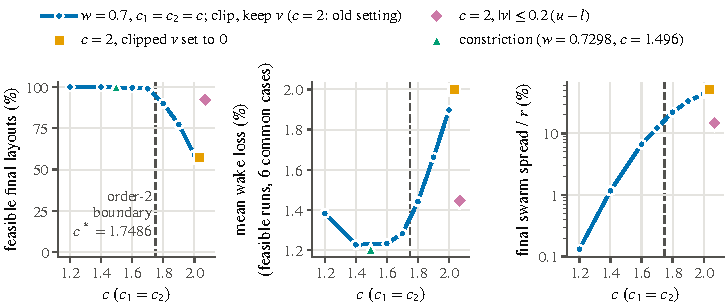
\includegraphics[width=\textwidth]{figures_mpce/csweep.pdf}
\caption{Stand-alone PSO with $w=0.7$ and $c_1=c_2=c$ on the 12 split cases $\times$ 30 seeds (6{,}030 evaluations, random starts; line with circles), the old setting ($c=2$) with two other bound-handling rules (clipped velocity components set to zero, squares; velocity clamping $|v|\le v_{\max}=0.2\,(u-l)$, diamonds; drawn slightly to the right of $c=2$), and the constriction setting (triangles; $w=0.7298$, $c=1.49618$; stored runs of the main comparison, spread not logged). The dashed vertical line is the order-2 stability boundary $c^\ast=12(1-w^2)/(7-5w)=1.7486$ of Proposition~\ref{prop:S-pso-stability} (stagnation, no bounds). Left: feasible final layouts (\% of 360 runs). Middle: mean wake loss of the feasible runs, averaged over the 6 cases in which every setting has at least 15 feasible runs. Right: median final swarm spread (mean over particles of the RMS turbine distance to the global best), relative to the farm radius (log scale). All settings start from the same seeded initial swarm. Values: Table~\ref{tab:S-csweep}.}
\label{fig:S-csweep}
\end{figure*}

\begin{table*}[!t]
\centering
\caption{PSO coefficient sweep and bound handling (12 split cases $\times$ 30 seeds, 6{,}030 evaluations, random starts). Feasible: final layouts feasible (\% of 360 runs); $N\ge10$: the same for the 180 runs with $N=10, 12, 15$; qualified: cases with at least 15 of 30 feasible runs; $L$: mean wake loss (\%) of the feasible runs, averaged over the 6 cases in which every setting is qualified; $L_{12}$: the same over all 12 cases (only for settings qualified in all 12); rank: average rank over the 12 cases among the ten settings (feasibility-aware rule of the main comparison: settings with fewer than 15 feasible runs rank below all qualified ones); spread: median final swarm spread relative to the radius (\%); clipped: coordinates leaving the box per iteration (\%, iterations 1--200); feasible evals: particle evaluations with a feasible layout in iterations 101--200 (\%). The row $c=2.0$ reproduces the stored runs of the old setting bit for bit; the constriction row is the stored PSO data of the main comparison (dynamics not logged). Order-2: whether $(w,c)$ satisfies the order-2 condition of Proposition~\ref{prop:S-pso-stability} ($c<\NSBoundC$ at $w=0.7$), which assumes no velocity clamping. For every setting and seed, the final layout is feasible in Data Set~I if and only if it is feasible in Data Set~II (same geometry; the penalty dominates while a layout is infeasible), so the feasibility columns rest on 6 geometries $\times$ 30 seeds.}
\label{tab:S-csweep}
\scriptsize\setlength{\tabcolsep}{3.5pt}
\resizebox{\ifdim\width>\textwidth\textwidth\else\width\fi}{!}{%
\begin{tabular}{cclcccccccccc}
\toprule
$w$ & $c$ & Bound handling & Order-2 & Feasible (\%) & $N\ge10$ (\%) & Qualified & $L$ (\%) & $L_{12}$ (\%) & Rank & Spread (\%) & Clipped (\%) & Feas.\ evals (\%) \\
\midrule
0.7 & 1.2 & clip, keep $v$ & yes & 100.0 & 100.0 & 12 & 1.38 & 3.05 & 5.42 & 0.1 & 0.5 & 80.4 \\
0.7 & 1.4 & clip, keep $v$ & yes & 100.0 & 100.0 & 12 & 1.23 & 2.77 & 2.50 & 1.2 & 0.9 & 69.9 \\
0.7 & 1.6 & clip, keep $v$ & yes & 99.4 & 99.2 & 12 & 1.23 & 2.77 & 2.33 & 6.6 & 1.9 & 41.5 \\
0.7 & 1.7 & clip, keep $v$ & yes & 98.9 & 98.3 & 12 & 1.28 & 2.93 & 3.58 & 12.2 & 2.9 & 25.4 \\
0.7 & 1.8 & clip, keep $v$ & no & 90.0 & 85.0 & 12 & 1.44 & 3.37 & 6.17 & 22.1 & 4.3 & 13.1 \\
0.7 & 1.9 & clip, keep $v$ & no & 77.2 & 65.8 & 10 & 1.66 & -- & 7.83 & 33.4 & 6.3 & 5.6 \\
0.7 & 2.0 & clip, keep $v$ & no & 58.9 & 38.3 & 6 & 1.90 & -- & 9.17 & 43.6 & 8.7 & 2.6 \\
\midrule
0.7 & 2.0 & clip, $v\gets0$ & no & 57.2 & 35.8 & 6 & 2.00 & -- & 9.83 & 50.8 & 8.8 & 2.5 \\
0.7 & 2.0 & $|v|\le v_{\max}$, clip & no & 92.2 & 88.3 & 12 & 1.45 & 3.42 & 6.42 & 14.7 & 1.6 & 11.8 \\
0.7298 & 1.496 & clip, keep $v$ & yes & 100.0 & 100.0 & 12 & 1.20 & 2.69 & 1.75 & -- & -- & -- \\
\bottomrule
\end{tabular}}
\end{table*}

\endgroup
\emph{Coefficient sweep.} A comparison of two settings cannot show whether the order-2 boundary marks where this PSO fails, nor separate the step size from the bound handling. A sweep of $c_1=c_2=c$ at $w=0.7$ (Fig.~\ref{fig:S-csweep} and Table~\ref{tab:S-csweep}; \NSCases{} cases of the split study $\times$ \NSSeeds{} seeds, \NSRuns{} runs per setting, 6,030 evaluations, random starts; $c=2.0$ reproduces the stored runs of the old setting bit for bit) shows that the boundary $c^\ast=\NSBoundC$ marks approximately where this PSO starts to fail: at least \NSFeasBelow\% of the runs are feasible for $c\le\NSCBelow$, then feasibility declines progressively (\NSFeasAbove\% at $c=\NSCAbove$, \NSFeasCTwoZero\% at 2.0); velocity clamping raises it to \NSFeasVMax\%, still worse than constriction in all \NSLossCasesVMaxConstr{} cases.
% CHECK-CSWEEP [S01] c = 2.0 reproduces the stored old-setting runs; [S02] c <= 1.7 >= 98 % feasible; [S03] c = 1.8 > 1.9 > 2.0; [S04] decline starts in the step containing c*; [S05] progressive, no jump; [S10] vmax >= 90 %; [S11] vmax worse than constriction in all 12 cases (never "causes")
The left panel of Fig.~\ref{fig:S-csweep} has no step at $c^\ast$: the loss of feasibility begins in the step from 1.7 to 1.8, which contains $c^\ast$, and accelerates beyond it (\NSFeasCOneEight\%, \NSFeasCOneNine\% and \NSFeasCTwoZero\% at $c=1.8$, 1.9 and 2.0). The other two panels change smoothly through $c^\ast$. The final swarm spread grows monotonically with $c$, by about an order of magnitude from $c=1.4$ to 1.7, on the stable side (\NSSpreadCOneFour\% of the radius at $c=1.4$, \NSSpreadCOneSeven\% at 1.7, \NSSpreadCTwoZero\% at 2.0), and the mean wake loss of the feasible runs rises already from $c=1.6$ to 1.7 (lower at $c=1.6$ in \NSLossBetterSixSeven{} of \NSLossCasesSixSeven{} cases, $p=\NSLossPSixSeven$), then steeply beyond $c^\ast$ (from 1.7 to 1.8 in all \NSLossCasesSevenEight{} cases). Too small coefficients also cost quality: $c=1.2$, whose final swarm spread is only \NSSpreadCOneTwo\% of the radius, has a higher mean wake loss than $c=1.4$ and 1.6. The boundary is therefore a useful marker of where the steps become too large for this bounded problem, but the sweep does not show that crossing it causes the failure; the degradation is gradual and begins on the stable side.
% CHECK-CSWEEP [S06] spread grows monotonically, >= 5x from 1.4 to 1.7; [S07] loss degrades on the stable side, c = 1.6 beats 1.7 in >= 10 of 12 (Wilcoxon p < 0.05); [S08] 1.7 -> 1.8 worsens the loss in all 12 cases; [S14] c = 1.2 worse than 1.4 and 1.6
The sweep also separates the step size from the bound handling. Setting the velocity components of clipped coordinates to zero does not rescue the old setting (\NSFeasVZero\% feasible, against \NSFeasCTwoZero\%), whereas velocity clamping, $\lvert v\rvert\le\NSVmaxFrac\,(u-l)$, which limits the step length itself, brings it to about the level of $c=1.8$ without clamping. The deficit of the old setting therefore comes mainly from its large steps, not from the way the bounds are enforced. The constriction setting has the best average rank of the ten settings of Table~\ref{tab:S-csweep} (\NSRankConstr), and $c=1.4$ at $w=0.7$ is as feasible and not significantly different in wake loss ($p=\NSLossPFourConstr$), which suggests that the step size, not the constriction form itself, is what matters. Feasibility is identical in the two data sets for every setting and seed (same geometry), so the feasibility columns rest on six geometries $\times$ \NSSeeds{} seeds.
% CHECK-CSWEEP [S09] zeroing clipped velocities no rescue; [S12] vmax indistinguishable from c = 1.8; [S13] constriction best rank, c = 1.4 not different; [S15] feasibility identical in Data Sets I and II

Table~\ref{tab:baseline} shows the effect on a comparison. It ranks an eight-method pool, the methods of Table~\ref{tab:friedman68} with LX-SSA-VNS instead of PSO-VNS, once with each PSO setting (all other methods use identical runs): with the old setting, \NBaseOldBest{} ranks first and PSO only in position \NBaseOldPSOPos{}, behind both salp-swarm hybrids; with the constriction setting, \NBaseNewBest{} ranks first, ahead of every salp-swarm method (standard coefficients~\cite{Clerc2002}; none of the methods was tuned on these cases). The reversal holds at 6,030 evaluations; on the six largest cases at 120,030, SSA-VNS ranks ahead of PSO (\NBudRankSSAVNSOneTwentyK{} vs.\ \NBudRankPSOOneTwentyK; Section~\ref{sec:budget}). The old setting thus makes the methods compared with it, including our own LX-SSA, appear stronger than they are.
% CHECK-FINAL [C27]: same pool: old setting SSA-VNS (1.99) and LX-SSA-VNS (2.65) ahead of PSO (5.04, NBaseOldPSOPos); constriction PSO ahead of every salp-swarm method (NBaseNewBest = PSO)
% CHECK-FINAL [C45]: at 120,030 evaluations SSA-VNS ranks ahead of PSO on the six largest cases

\subsection{Overall Comparison}
\label{sec:overall}
%% generated by mpce_results.py -- do not edit by hand
\begin{table*}[!t]
\centering
\caption{Case-level analysis over the 68 benchmark cases. Ranks of the mean feasible objective within each case (1 = best); a method with fewer than 15 feasible runs out of 30 in a case is ranked below all other methods, by its number of feasible runs (``$<$15'': number of such cases). Friedman $\chi^2_F=174.4$ (6 d.f.), $p=5.29\times10^{-35}$; Iman--Davenport $F_F=50.0$, $p=8.06\times10^{-46}$. $p_z$: Holm-adjusted $p$ of the average-rank $z$ test against SSA-VNS (best-ranked method: SSA-VNS). Because mean-rank post hoc tests depend on the pool of compared methods \cite{Benavoli2016}, pairwise two-sided Wilcoxon signed-rank tests on the per-case mean wake losses (\%) are also given: $p_W$ (Holm-adjusted over the 6 comparisons), matched-pairs rank-biserial correlation $r_{\rm rb}$ (positive = SSA-VNS better) and mean difference $\overline{\Delta L}$ of the wake loss (percentage points, SSA-VNS minus method, over the cases where both methods have at least 15 feasible runs). ``Best'': cases in which the method alone ranks first; ``Feas.'': percentage of feasible runs.}
\label{tab:friedman68}
\scriptsize\setlength{\tabcolsep}{3pt}
\begin{tabular}{lcccccccc}
\toprule
Method & Avg.\ rank & Best & Feas.\ (\%) & $<$15 & $p_z$ & $p_W$ & $r_{\rm rb}$ & $\overline{\Delta L}$ (pp) \\
\midrule
SSA-VNS & 1.74 & 37 & 99.6 & 0 & -- & -- & -- & -- \\
VNS & 2.97 & 8 & 100.0 & 0 & $8.55\times10^{-4}$ & $5.49\times10^{-7}$ & +0.77 & $-0.135$ \\
SSA & 3.88 & 0 & 97.6 & 2 & $1.36\times10^{-8}$ & $2.27\times10^{-10}$ & +0.96 & $-0.294$ \\
PSO & 4.17 & 3 & 86.0 & 8 & $1.52\times10^{-10}$ & $1.44\times10^{-9}$ & +0.92 & $-0.337$ \\
MS-SLSQP & 4.47 & 11 & 99.9 & 0 & $6.18\times10^{-13}$ & $3.34\times10^{-5}$ & +0.58 & $-0.112$ \\
LX-SSA & 4.69 & 0 & 96.9 & 2 & $7.40\times10^{-15}$ & $5.53\times10^{-11}$ & +1.00 & $-0.447$ \\
DE & 6.08 & 0 & 71.4 & 18 & $5.39\times10^{-31}$ & $7.74\times10^{-11}$ & +1.00 & $-0.680$ \\
\bottomrule
\end{tabular}
\end{table*}

%% generated by mpce_results.py -- do not edit by hand
\begin{table}[!t]
\centering
\caption{Pairwise outcome of PSO-VNS against each method: number of cases in which PSO-VNS is significantly better / not significantly different / significantly worse (two-sided Wilcoxon signed-rank test on 30 seed-paired runs, Holm-adjusted over the 7 comparisons of each case, $\alpha=0.05$; infeasible runs rank below all feasible runs). Last row: median over the cases of the rank-biserial correlation $r_{\rm rb}$ (positive = PSO-VNS better).}
\label{tab:wtl}
\scriptsize\setlength{\tabcolsep}{2.5pt}
\begin{tabular}{llcccccccc}
\toprule
DS & $r$ (m) & Cases & PSO & SSA-VNS & SSA & LX-SSA & DE & VNS & MS-SLSQP \\
\midrule
I & 500 & 9 & 0/8/1 & 6/3/0 & 8/1/0 & 8/1/0 & 7/2/0 & 6/3/0 & 7/2/0 \\
I & 750 & 11 & 1/8/2 & 9/2/0 & 10/1/0 & 10/1/0 & 9/2/0 & 8/3/0 & 10/1/0 \\
I & 1000 & 14 & 3/11/0 & 9/5/0 & 12/2/0 & 12/2/0 & 12/2/0 & 12/2/0 & 12/2/0 \\
II & 500 & 9 & 3/5/1 & 7/2/0 & 7/2/0 & 8/1/0 & 7/2/0 & 7/1/1 & 8/1/0 \\
II & 750 & 11 & 2/9/0 & 8/3/0 & 10/1/0 & 10/1/0 & 9/2/0 & 8/3/0 & 9/2/0 \\
II & 1000 & 14 & 5/9/0 & 10/4/0 & 12/2/0 & 12/2/0 & 12/2/0 & 10/4/0 & 13/1/0 \\
\midrule
All & & 68 & 14/50/4 & 49/19/0 & 59/9/0 & 60/8/0 & 56/12/0 & 51/16/1 & 59/9/0 \\
$\tilde r_{\rm rb}$ & & & +0.08 & +0.72 & +0.98 & +0.97 & +1.00 & +0.84 & +0.98 \\
\bottomrule
\end{tabular}
\end{table}


Over the eight methods (Table~\ref{tab:friedman68}), the Friedman test \NFriedVerb{} the hypothesis of equal performance ($\chi^2_F=\NFriedChi$, $p=\NFriedP$; Iman--Davenport $F_F=\NImanF$, $p=\NImanP$). PSO-VNS has the best average rank (\NRankPSOVNS), alone ranks first in \NSoleBestPSOVNS{} cases, and stays first when the final layouts are re-evaluated with 5$^\circ$ or 1$^\circ$ direction sub-bins (1$^\circ$: \NFRankPSOVNSOne; Section~\ref{sec:robustness}). In the Holm-adjusted post hoc tests ($p_z$ in Table~\ref{tab:friedman68}; tied ranks make them conservative), PSO-VNS ranks significantly better than \NPostHocSigList{}, but not than \NPostHocNonSigList{} ($p_{\rm Holm}=\NPostHocNonSigP$). The rank order and these conclusions are unchanged for thresholds of \NXThrList{} feasible runs; significant comparisons with PSO-VNS favor the same method in each of the \NXClusters{} clusters, and leaving out one cluster changes none of them (Tables~\ref{S-tab:X-threshold}--\ref{S-tab:X-loco}).
% CHECK-FINAL [C01]: main.friedman.best_ranked == PSOBV; [C02]: p < 0.05 (verb generated: \NFriedVerb); [C03]: p_holm_vs_focus: only PSOC >= 0.05
% CHECK-DIR [F06]: PSO-VNS best average rank with 5-deg and 1-deg sub-bins (\NFRankPSOVNSOne)
% CHECK-EXTRA [X02][X03][X05]-[X09] six thresholds 1-30; [X11] clusters 6/6 same direction for comparisons with PSO-VNS; [X14] LOCO changes only \NXLocoChanged (not a PSO-VNS comparison), PSO-VNS always best

\begin{figure}[!t]
\centering
\pipefig{0.55\textwidth}{figures_mpce/avg_ranks.pdf}{5cm}
\caption{Average rank of the eight methods of the main comparison over the 68 benchmark cases (feasibility-aware ranking of Table~\ref{tab:friedman68}; 1 = best).}
\label{fig:ranks}
\end{figure}
% CHECK (pipeline): avg_ranks.pdf is drawn from the same ranks as tab:friedman68 (\NRankPSOVNS ... \NRankDE)
Fig.~\ref{fig:ranks} shows the average ranks. The two PSO-based methods lead with a small gap between them (\NRankPSOVNS{} and \NRankPSO), and the gap to the next method, SSA-VNS (\NRankSSAVNS), is much larger. VNS alone (\NRankVNS) ranks ahead of SSA (\NRankSSA), MS-SLSQP (\NRankSLSQP) and LX-SSA (\NRankLXSSA), and DE ranks last (\NRankDE). The ranking is feasibility-aware: a method with fewer than 15 feasible runs in a case ranks below all qualified methods there, so the rank of DE, which is feasible in \NFeasDE\% of its runs, reflects its feasibility as much as its wake loss. Both hybrids rank ahead of their first phase alone (PSO-VNS ahead of PSO, SSA-VNS ahead of SSA) and of VNS alone; the component analysis of Section~\ref{sec:ablation} asks which phase is responsible.
% CHECK (pipeline): rank values from tab:friedman68; [C01] PSO-VNS best; DE feasibility \NFeasDE (CHECK-FINAL [C08])

Against SSA-VNS, PSO-VNS is significantly better in \NWtlSSAVNSW{} cases and never worse ($p_{\rm Holm}=\NPWSSAVNS$). Against SSA, LX-SSA, DE, VNS and MS-SLSQP (untuned DE; finite-difference gradients), it is significantly better in most cases; \NLossesPhrase. PSO-VNS is more reliable in reaching feasibility on the Horns Rev~1 block with random starts (\NHRFeasPSOVNS{} vs.\ \NHRFeasPSO{}, McNemar $p=\NXHRMcNemarP$; Section~\ref{sec:hornsrev-site}) and ranks best on the six largest cases at all three budgets (exploratory; Section~\ref{sec:budget}). The leading methods depend on the conditions: from feasible starts, \NFbFeasBestRank{} ranks first (Section~\ref{sec:feasinit}); under the Gaussian wake, \NBestGauss{} ranks narrowly ahead of PSO-VNS with 15$^\circ$ bins but not with 1$^\circ$ sub-bins (Section~\ref{sec:gaussian}).
% CHECK-FINAL [C06]: wtl.SSABV.L == 0; [C07]: better than SSA, LX-SSA, DE, VNS, MS-SLSQP in most cases; [C08]/[C20]: Horns Rev PSO-VNS 30/30, PSO < 30/30; [C29]: six largest cases best at all budgets; [C28]: feasible-start BVNS best; [C22]: Gauss 15 deg PSOC first, PSOBV second
% CHECK-EXTRA [X52] McNemar (one site, random starts); CHECK-DIR [F06] best rank 15/5/1 deg; [F09] Gaussian: PSO first at 15 deg, PSO-VNS at 1 deg

\begin{figure*}[!t]
\centering
\pipefig{0.92\textwidth}{figures_mpce/wakeloss_vs_n.pdf}{8cm}
\caption{Mean wake loss (\% of the wake-free benchmark objective) of the feasible runs versus the prescribed number of turbines $N$, for each farm and wind data set (30 runs of 6,030 evaluations, random initialization). A point is drawn only when the method has at least 15 feasible runs in that case, so a curve (mostly DE) stops where the method has too few feasible runs.}
\label{fig:wakeloss}
\end{figure*}
The wake loss grows with $N$, falls as the farm becomes larger, and is higher for the broader wind rose of Data Set~II (Fig.~\ref{fig:wakeloss}). PSO-VNS ends feasible in all runs (DE: \NFeasDE\%). In the densest cases (500~m, $N=10$), the global best of the PSO phase is feasible at the switch in only \NDenseSwitchFeas\% of the runs, but all runs are feasible after the VNS phase.
% CHECK-FINAL [C42]: case-mean wake loss grows with N, falls with r, DS II >= DS I; [C08]: feasible_pct.PSOBV == 100; [C24]: dense_500_10 feasible at switch < 100
Fig.~\ref{fig:wakeloss} also shows where the cases differ in difficulty. For the smallest $N$, all methods reach almost no wake loss, because a few turbines can be placed so that they hardly shade each other in any direction; these cases cannot separate the methods. The curves fan out as $N$ grows and the turbines must share a fixed disc: the losses rise faster in the small farm than in the large one, and faster under the broad rose of Data Set~II, in which more directions carry wind, so that wakes are harder to avoid. The ranking of Fig.~\ref{fig:ranks} is thus decided mainly by the larger layouts, in which PSO-VNS and PSO lie close together at or near the bottom of each panel; DE loses feasibility first as the layouts become denser.
% CHECK-FINAL [C42] (monotone in N, r, data set); curves: wakeloss_vs_n.pdf from the case means of tab:friedman68 runs

\begin{figure*}[!t]
\centering
\pipefig{0.7\textwidth}{figures_mpce/ablation_convergence.pdf}{6.6cm}
\caption{Convergence of the \NAblNVar{} component-analysis variants (Table~\ref{tab:ablation}) for the largest turbine count of each farm: median best feasible wake loss over 30 runs versus evaluations. PSO-VNS and PSO coincide up to 3,030 evaluations (dotted line), where PSO-VNS switches to VNS. Curves of the main comparison: Fig.~\ref{S-fig:S-conv-max} of the supplementary material.}
\label{fig:conv-max}
\label{fig:ablation}
\end{figure*}
% CHECK (pipeline count): \NAblNVar = variants of tab:ablation = curves of ablation_convergence.pdf; [C58] ranks

After the switch, both keep improving (Fig.~\ref{fig:conv-max}): the VNS phase removes on average \NPhTwoMean\% (median \NPhTwoMedian\%) of the wake loss left after the PSO phase and repairs \NPhTwoMadeFeas{} runs infeasible at the switch, whereas continuing PSO for the same 3,000 evaluations removes \NPsoContMean\% (median \NPsoContMedian\%).
% CHECK-FINAL [C10]: phase2 PSOBV.mean >= PSOC_continued.mean > 0 ("both keep improving")
The two ways of spending the second half of the budget are therefore nearly equally productive on average. They differ in what they do: continued PSO keeps contracting the swarm around $\mathbf G$, whereas the VNS phase performs a local (compass) search from $\mathbf G$ along the coordinate directions; the next subsection shows that this difference matters in some cases and in opposite directions.

\subsection{PSO-VNS versus PSO}
\label{sec:psovns-pso}
Against PSO, PSO-VNS is significantly better in \NWtlPSOW{} cases, tied in \NWtlPSOT{} and worse in \NWtlPSOL{} (run level, Table~\ref{tab:wtl}). The case means do not differ significantly ($\overline{\Delta L}=\NCmPSOVNSvsPSODL$~pp, $p=\NCmPSOVNSvsPSOP$; Hodges--Lehmann estimate \NXHLPSOVNSvsPSO~pp). Whether the difference is negligible at the post hoc margin $\pm\NEqMargin$~pp depends on the level of inference (Table~\ref{tab:X-equiv-levels}): on this fixed benchmark (seed level), PSO-VNS has a small significant advantage inside the margin (90\% CI \NXEqSeedPSOVNSvsPSOCI); over exchangeable cases the two are equivalent (\NXEqCasePSOVNSvsPSOCI, TOST $p=\NXEqCasePSOVNSvsPSOP$, minimal margin \NXEqCasePSOVNSvsPSOMin); over farm clusters, equivalence is not shown (CR2 \NXEqClustPSOVNSvsPSOCI, minimal margin \NXEqClustPSOVNSvsPSOMin). In the Bayesian signed-rank test, practical equivalence is the most probable outcome (posterior probability \NBayPSOVNSvsPSORope; posterior means \NXBayMeanPSOVNSvsPSOLeft/\NXBayMeanPSOVNSvsPSORope/\NXBayMeanPSOVNSvsPSORight{} for PSO-VNS better by more than the margin/equivalent/PSO better). The margin corresponds to \NXMarginMWhTurbDsI{} (Data Set~I) and \NXMarginMWhTurbDsII~MWh/yr (Data Set~II) per turbine, the mean gain of PSO-VNS to \NXEnPSOVNSvsPSOMWhTurb~MWh/yr per turbine (\NXEnPSOVNSvsPSOPct\% of AEP). Spread and worst run do not differ ($p=\NSdP$, \NWorstP).
% CHECK-FINAL [C04]: PSOC: W >= L, mean loss PSOBV < PSOC, case-mean p >= 0.05; [C49]: case-level 90% CI inside +-m, P(rope most probable) printed via \NBayPSOVNSvsPSORope; [C52]: SD p and worst-run p >= 0.05
% CHECK-EXTRA [X39] seed and case level equivalent, cluster level not; [X40] seed-level CI excludes 0 inside m; [X41] minimal margins seed < case < m < cluster; [X48] Bayesian wording + posterior means; [X50] HL near 0; [X56] margin 4.1/2.1 MWh/yr per turbine, mean gain 0.2; [X25] energy < 0.05 % AEP

\begingroup\swResRefs
\SuppTable{tab:X-equiv-levels}
\begin{figure}[!t]
\centering
\pipefig{0.6\textwidth}{figures_mpce/equiv_curve.pdf}{5cm}
\caption{Equivalence curve of PSO-VNS vs.\ PSO: TOST $p$ value versus the equivalence margin $m$ (pp of wake loss) at three levels of inference (Table~\ref{tab:X-equiv-levels}): seed level (fixed benchmark; bootstrap of the seed-paired runs within every case), case level (bootstrap over the 68 cases, as Table~\ref{tab:equivalence}) and cluster level (six farm clusters; CR2 cluster-robust $t$ with 5 d.f., and the restricted wild-cluster bootstrap). Dotted lines: $\alpha=0.05$ and the margin $m=\NEqMargin$~pp. The dots mark the minimal margins $m_{\min}$, at which a curve crosses $\alpha$; equivalence holds at every margin to the right of the dot. The bootstrap curves stop at their resolution limit $1/10{,}001$.}
\label{fig:equiv-curve}
\end{figure}
\endgroup
% CHECK-EXTRA [X57] equiv_curve.pdf generated in the same run; [X41] minimal margins seed < case < m < cluster
The three levels answer three different questions, and Table~\ref{tab:X-equiv-levels} gives all of them for every pair of the paper. The \emph{seed level} treats the 68 cases as fixed and only the run-to-run variability as random: would new seeds on this benchmark reproduce the difference? The \emph{case level} treats the cases as exchangeable draws from a population of similar cases, and the \emph{cluster level} accounts for the structure of the benchmark, six (data set, radius) clusters with nested $N$, and asks whether the result carries over to new farms and wind roses; with only six clusters its intervals are wide. For PSO-VNS versus PSO the minimal margin at which equivalence holds therefore grows with the scope of the question: \NXEqSeedPSOVNSvsPSOMin~pp at the seed level, \NXEqCasePSOVNSvsPSOMin~pp at the case level and \NXEqClustPSOVNSvsPSOMin~pp at the cluster level (Fig.~\ref{fig:equiv-curve}), with the margin \NEqMargin~pp between the second and the third. Because this margin was set after the primary analysis and lies only slightly above the case-level minimal margin, Fig.~\ref{fig:equiv-curve} shows the whole TOST $p$ curve, so that readers can apply their own threshold; the seed-level interval, which excludes zero, also shows that ``equivalent'' and ``different'' are not contradictory here: the two methods differ reproducibly on this benchmark, but by less than the margin. For the other pairs of the main comparison the whole interval lies beyond the margin at every level, so that their verdicts do not depend on the margin or the level; equivalence at the cluster level is shown for no pair.
% CHECK-EXTRA [X39]-[X41]; [X55] no pair equivalent at the cluster level; main-comparison pairs other than PSO: whole 90% CI beyond -m at all three levels (tab:X-equiv-levels, m_min > m)

\begingroup\swResRefs\swResWrapNotes
\SuppTable{tab:X-heterogeneity}
\endgroup
The average hides case-level differences in both directions: \NXHetBeyondPSOVNS{} cases favor PSO-VNS by more than the margin (by up to \NXHetMaxPSOVNS~pp) and \NXHetBeyondPSO{} favor PSO (up to \NXHetMaxPSO~pp; Table~\ref{tab:X-heterogeneity}). The two are equivalent for $N<10$ (\NXEqSmallN{} cases, 90\% CI \NXEqSmallCI) but not for $N\ge10$ (\NXEqLargeMean~pp, \NXEqLargeCI) or on the \NXEqNontrivialN{} cases with a wake loss of at least \NXTrivialLoss~pp (\NXEqNontrivialCI). They follow a data set $\times$ density crossover (density $\phi=\NXDensDef$; stated after review, exploratory; interaction $p=\NXDensInterP$): as $\phi$ grows, PSO-VNS gains in Data Set~II (slope \NXDensSlopeDsII~pp, $p=\NXDensPDsII$) and PSO in Data Set~I (\NXDensSlopeDsI~pp, $p=\NXDensPDsI$). In the post hoc subgroup Data Set~II, $N\ge10$, PSO-VNS has the lower mean wake loss in \NCmPSOVNSvsPSOdsIILargeWins{} of \NCmPSOVNSvsPSOdsIILargeN{} cases ($p_{\rm Holm}\le\NXHolmPSOVNSvsPSOdsIILargeP$ over all \NXMultN{} case-mean Wilcoxon tests; \NXEnPSOVNSvsPSOdsIILargePct\% of AEP); all \NXHetDsINPSO{} Data Set~I cases beyond the margin favor PSO. With 1$^\circ$ sub-bins, PSO-VNS is slightly but significantly better than PSO ($\overline{\Delta L}=\NFPairMeanOne$~pp, 90\% CI \NFPairCIOne; Table~\ref{S-tab:F-equiv}).
% CHECK-EXTRA [X43] 11/8 beyond +-m, max 0.41/0.27; [X44] N < 10 equivalent, N >= 10 not; [X45] non-trivial cases not equivalent; [X47] data set x density crossover (exploratory, stated after review); [X19] DS II N >= 10 survives all-family Holm ("<=", R5 O13); [X27] DS II N >= 10 ~0.2 % AEP
% CHECK-FINAL [C32]: DS II N >= 10 case-mean wins > losses
% CHECK-DIR [F10]: 1-deg PSO-VNS - PSO CI below 0, not equivalent; [F14]: DS II N >= 10 advantage survives at 1 deg

Table~\ref{tab:X-heterogeneity} shows why the average verdict must be read together with its composition. Of the 68 cases, \NXEqSmallN{} have $N<10$, and in the \NXEqTrivialN{} cases in which PSO-VNS leaves a wake loss below \NXTrivialLoss~pp, no case differs by more than the margin (90\% CI \NXEqTrivialCI): these easy cases, in which both methods find almost wake-free layouts (Fig.~\ref{fig:wakeloss}), pull the average towards zero. Every case beyond the margin is non-trivial, and on the \NXEqNontrivialN{} non-trivial cases the interval \NXEqNontrivialCI{} is not inside $\pm\NEqMargin$~pp, so that equivalence is not shown where the comparison has something to decide. The differences are not scattered at random either: \NXHetClBeyond{} of the \NXClustersNum{} cluster means of PSO-VNS $-$ PSO lie beyond the margin, \NXHetClBeyondPSOVNS{} in favor of PSO-VNS and \NXHetClBeyondPSO{} in favor of PSO (Data Set~II, 500~m and 1000~m: \NXHetClDsIIFive{} and \NXHetClDsIIThousand~pp; Data Set~I, 500~m: \NXHetClDsIFive~pp). The pattern behind this is the crossover: in Data Set~II, \NXHetDsIINPSOVNS{} cases beyond the margin favor PSO-VNS, the larger layouts of all three farms, and \NXHetDsIINPSO{} favors PSO, whereas in Data Set~I all \NXHetDsINPSO{} such cases favor PSO, all of them dense layouts in the 500-m and 750-m farms (Table~\ref{S-tab:X-beyond}). The density variable was defined after the review and before this test was run, and the analysis does not identify a cause, so we report the crossover as an exploratory pattern and a hypothesis for designed experiments, not as a property of the two algorithms. For the practical question the result is clear enough: PSO-VNS does not dominate a well-configured PSO; it is at least as good on average over this benchmark, gains in the larger layouts of the broad rose of Data Set~II, and loses in dense layouts under the rose of Data Set~I.
% CHECK-EXTRA [X44] N < 10 (48 cases) equivalent; [X45] trivial cases equivalent, every case beyond the margin non-trivial, non-trivial not equivalent; [X46] 3 of 6 cluster means beyond +-m in opposite directions (2 PSO-VNS, 1 PSO; DS I 500 m, DS II 1000 m); [X47] DS I cases beyond the margin all favor PSO and are dense, DS II 11 favor PSO-VNS, 1 favors PSO (exploratory, stated after review)
